\section{MPC Formulation}

\subsection{Overview}
\begin{frame}{Overview}
  \begin{itemize}
    \item \alert{Quadratic} cost function
      \begin{equation*}
        J = \sum_{i=1}^p
        \tps{\left( \Delta y_i - \Delta y_i^\text{ref}\right)}
        W_y
        {\left( \Delta y_i - \Delta y_i^\text{ref}\right)}
        +\sum_{i=1}^m
        \tps{\left( \Delta u_i\right)}
        W_u
        {\left( \Delta u_i\right)}
      \end{equation*}
    \item \alert{Linearized}, discretized, augmented formulation
      \begin{align*}
        \text{s.t. }\gpio{xaug} ={}&
        \ga{augsys-mats}
        \gpi{xaug} 
        + 
        \gb{augsys-mats}
        \gpi{deltau}
        + \g{fcurr}\\
% y
        \gi{Delta} \g{ycurr} ={}& \gc{augsys-mats}
        \g{xaug}
      \end{align*}
    \item Input constraints (absolute value and rate)
      \begin{equation*}
        \begin{split}
          \text{s.t. } & \gi{Delta} U\ut{min} \leq \gi{Delta} U \leq \gi{Delta} U\ut{max}\\
          & \gi{Delta} U\ut{r,min} \leq A\ut{rate} \gi{Delta} U \leq \gi{Delta} U\ut{r,max}\\
        \end{split}
      \end{equation*}
  \end{itemize}


  % How is MPC implemented?\\
  % How is the cost function formulated?\\
  % How are the constraints implemented?
\end{frame}

\begin{frame}{Quadratic Program}
  \small
  \begin{equation*}
    \begin{split}
      & \argmin_{U}\ \frac{1}{2} \tps{\gi{Delta}U}\ H\ \gi{Delta}U + \tps{g} \gi{Delta} U\\
      \text{s.t. } & \gi{Delta} U\ut{min} \leq \gi{Delta} U \leq \gi{Delta} U\ut{max},
    \end{split}
  \end{equation*}
  \normalsize

  \begin{itemize}
    \item Dense formulation $\implies$ replace $\gi{Delta} Y$ terms using model
      \small
      \begin{equation*}
        \begin{split}
          \gi{Yk} & = \gi{prediction-matrices} \gi{Delta} \g{Uk} + \gii{prediction-matrices} \g{xaug} + \giii{prediction-matrices} \g{fcurr}\\
          & \qquad  \Downarrow\\
          H & = 2\left( W_u + \tps{\gi{prediction-matrices}}\ W_y\ \gi{prediction-matrices} \right)\\
          g & = 2\left( \g{xaug} \tps{\gii{prediction-matrices}} + \g{fcurr} \tps{\giii{prediction-matrices}} - \gi{Delta} \g{Yrefk} \right)W_y \gi{prediction-matrices}.\\
        \end{split}
      \end{equation*}
      \normalsize
    \item Solve using \qpoases{} active-set solver
  \end{itemize}

  % How is the QP setup?\\
  % What constraints are used?\\
  % What type of solver is used?
\end{frame}

\subsection{Distributed MPC}
\begin{frame}{Distributed MPC}
  \begin{itemize}
    \item One sub-controller for each compressor
      \small
      \begin{equation*}
        \begin{split}
          \gi{Yk} & = \gi{prediction-matrices} \gi{Delta} \g{Uk} + \gii{prediction-matrices} \g{xaug} + \giii{prediction-matrices} \g{fcurr} \structure{+ \g{prediction-uother}\gi{Uother}}\\
          & \qquad  \Downarrow\\
      % H\ut{dist.} & = 2\left( \gi{weights} + \tps{\gi{prediction-matrices}}\ \gii{weights}\ \gi{prediction-matrices} \right)\\
          H\ut{dist.} & = H\ut{cent.}\\
      % g\ut{dist.} & = 2\left( \g{xaug} \tps{\gii{prediction-matrices}} + \g{fcurr} \tps{\giii{prediction-matrices}} - \gi{Yrefk} \structure{+ \gi{Uother}\ \tps{\g{prediction-uother}}} \right)\gii{weights}\ \gi{prediction-matrices}\\
          g\ut{dist.} & = g\ut{cent.} \structure{+ \gi{Uother}\ \tps{\g{prediction-uother}} W_y\ \gi{prediction-matrices}}\\
        \end{split}
      \end{equation*}
      \normalsize
    \item Iterate, exchanging solution info between sub-controllers, to converge to optimal solution
  \end{itemize}

% \begin{equation}
  % \begin{split}
    % H\ut{distributed} & = 2\left( \gi{weights} + \tps{\gi{prediction-matrices}}\ \gii{weights}\ \gi{prediction-matrices} \right)\\
    % & = H\ut{centralized}\\
    % g\ut{distributed} & = 2\left( \g{xaug} \tps{\gii{prediction-matrices}} + \g{fcurr} \tps{\giii{prediction-matrices}} - \gi{Yrefk} + \gi{Uother}\ \tps{\g{prediction-uother}} \right)\gii{weights}\ \gi{prediction-matrices}\\
    % & = g\ut{centralized} + \gi{Uother}\ \tps{\g{prediction-uother}} \gii{weights}\ \gi{prediction-matrices}\\
  % \end{split}
  % \label{eq:mpc:distributed-qp-terms}
% \end{equation}
  % How does distributed MPC differ from centralized?\\
  % How is the cost function set up differently?\\
  % What extra terms does it have?
\end{slide}

\begin{slide}{Algorithm}
  \begin{figure}[H]
    \centering
    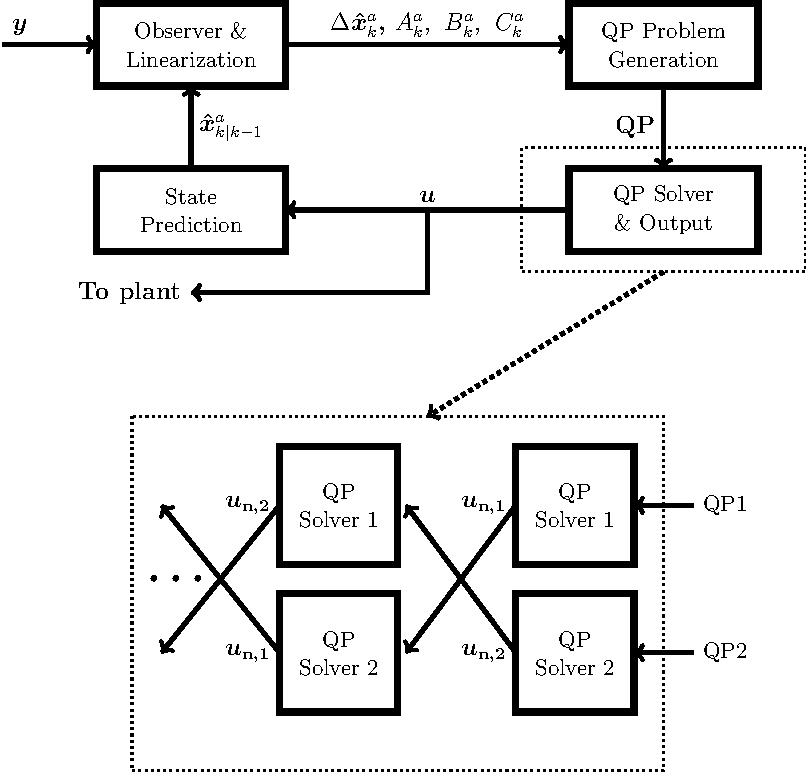
\includegraphics[width=.5\linewidth]{figures/algorithm.pdf}
  \end{figure}
  How does distributed MPC differ from centralized?\\
  How is the cost function set up differently?\\
  What extra terms does it have?
\end{frame}

\subsection{Implementation}
\begin{frame}{State Estimation}
  How are states estimated?\\
  Why a static observer matrix?
\end{frame}

\begin{frame}{Simulink}
  How is the Simulink model set up?\\
  Advantages/disadvantages
\end{frame}

\begin{frame}{C++}
  How is the C++ model set up?\\
  Computational speed advantages?
\end{frame}

